\let\negmedspace\undefined
\let\negthickspace\undefined
\documentclass[journal]{IEEEtran}
\usepackage[a5paper, margin=10mm, onecolumn]{geometry}
%\usepackage{lmodern} % Ensure lmodern is loaded for pdflatex
\usepackage{tfrupee} % Include tfrupee package

\setlength{\headheight}{1cm} % Set the height of the header box
\setlength{\headsep}{0mm}     % Set the distance between the header box and the top of the text

\usepackage{gvv-book}
\usepackage{gvv}
\usepackage{cite}
\usepackage{amsmath,amssymb,amsfonts,amsthm}
\usepackage{algorithmic}
\usepackage{graphicx}
\usepackage{textcomp}
\usepackage{xcolor}
\usepackage{txfonts}
\usepackage{listings}
\usepackage{enumitem}
\usepackage{mathtools}
\usepackage{gensymb}
\usepackage{comment}
\usepackage[breaklinks=true]{hyperref}
\usepackage{tkz-euclide} 
\usepackage{listings}
% \usepackage{gvv}                                        
\def\inputGnumericTable{}                                 
\usepackage[latin1]{inputenc}                                
\usepackage{color}                                            
\usepackage{array}                                            
\usepackage{longtable}                                       
\usepackage{calc}                                             
\usepackage{multirow}                                         
\usepackage{hhline}                                           
\usepackage{ifthen}                                           
\usepackage{lscape}
\usepackage{circuitikz}
\tikzstyle{block} = [rectangle, draw, fill=blue!20, 
    text width=4em, text centered, rounded corners, minimum height=3em]
\tikzstyle{sum} = [draw, fill=blue!10, circle, minimum size=1cm, node distance=1.5cm]
\tikzstyle{input} = [coordinate]
\tikzstyle{output} = [coordinate]


\begin{document}

\bibliographystyle{IEEEtran}
\vspace{3cm}

\title{4.8.27}
\author{AI25BTECH110031 \\ Shivam Sawarkar}
 \maketitle
% \newpage
% \bigskip
{\let\newpage\relax\maketitle}

\renewcommand{\thefigure}{\theenumi}
\renewcommand{\thetable}{\theenumi}
\setlength{\intextsep}{10pt} % Space between text and floats


\numberwithin{equation}{enumi}
\numberwithin{figure}{enumi}
\renewcommand{\thetable}{\theenumi}

\textbf{Question(4.8.27)} Find the equation of the plane passing through $(-1, 3, 2)$ and perpendicular to the planes $x + 2y + 3z = 5$ and $3x + 3y + z = 0$. \\ 

\textbf{Solution:} \\ 
Normals of the given planes are
\begin{align}
\vec{n_1} = \myvec{1 \\ 2 \\ 3},
\quad
\vec{n_2} = \myvec{3 \\ 3 \\ 1}.
\end{align}

Let the required plane have normal vector $\vec{n}$

Since it is perpendicular to both given planes:
\begin{align}
\vec{n_1}^\top \vec{n} = 0,
\quad
\vec{n_2}^\top \vec{n} = 0.
\end{align}

That is,
\begin{align}
\myvec{\vec{n_1} & \vec{n_2}}^\top\vec{n}=\myvec{0 \\ 0} \\ 
\myvec{
1 & 2 & 3 \\
3 & 3 & 1
}
\vec{n}
=
\myvec{
0 \\ 0
}.
\end{align}

Let
\begin{align}
\vec{n} = \myvec{a \\ b \\ c} \\ 
a + 2b + 3c = 0, \\
3a + 3b + c = 0.
\end{align}

From these, we get
\begin{align}
\vec{n} = t \myvec{7 \\ -8 \\ 3}, \quad t \in \mathbb{R}, \quad t \neq 0
\end{align}

Equation of plain is 
\begin{align}
    \vec{n}^\top\vec{x}=1
\end{align}
since point $\vec{p}=\myvec{-1 \\ 3 \\ 2}$ lies on the plain
\begin{align}
    \vec{n}^\top\vec{p}=1
\end{align}

Substituting,
\begin{align}
\myvec{7 & -8 & 3}
\myvec{x \\ y \\ z}
=
\myvec{7 & -8 & 3}\myvec{-1 \\ 3 \\ 2}.
\end{align}

\begin{align}
\myvec{7 & -8 & 3}
\myvec{x \\ y \\ z}
= -25
\end{align}

\begin{align}
\frac{-1}{25}\myvec{7 & -8 & 3}
\myvec{x \\ y \\ z}
=1 
\end{align}

\begin{align}
\vec{n}=\frac{-1}{25}\myvec{7 \\ -8 \\ 3}
\end{align}

\begin{align}
\vec{n}^\top \vec{x} = 1.
\end{align}

\begin{figure}[H]
    \centering
    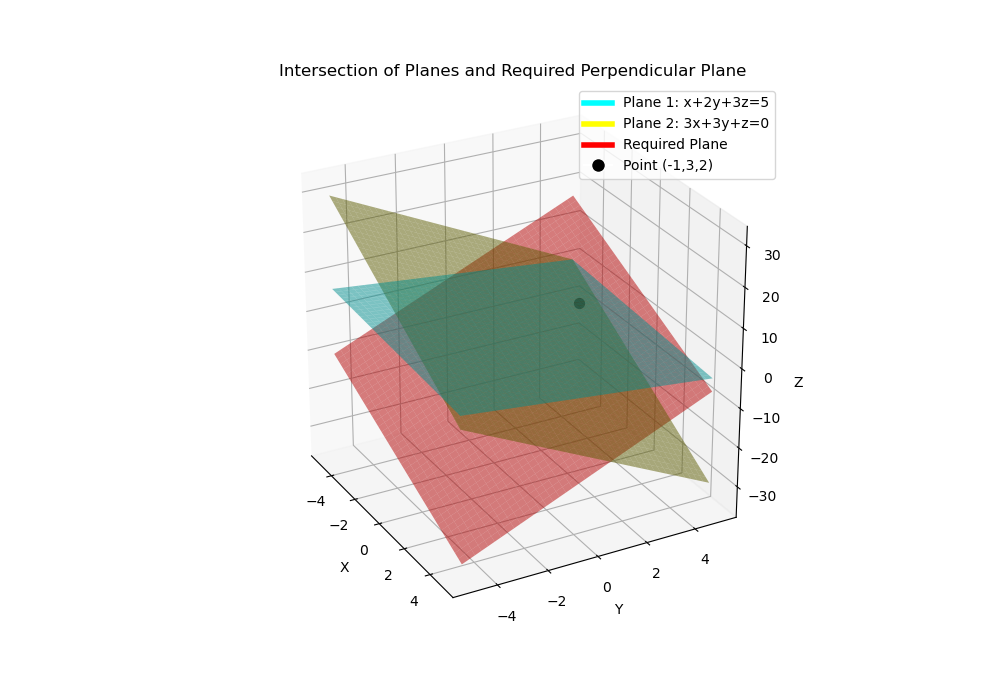
\includegraphics[width=0.8\linewidth]{figs/plot8.png}
    \caption{}
    \label{fig:placeholder}
\end{figure}









\end{document}